\documentclass{scrartcl}
\usepackage{pgfplots}
\usepackage{booktabs} % For better table formatting
\usepackage{calc}
\usepackage{Style_File}
\newcommand{\ad}[1]{a_{#1}^\dagger}
\usepackage{fancyhdr}
\usepackage{tikz-feynman}
\usepackage{tensor}
\usepackage{array}
\usepackage{lmodern}
\definecolor{violet}{rgb}{0.5,0.27,0.45}

\newcolumntype{P}[1]{>{\centering\arraybackslash}p{#1}}
% Recommended preamble:
\usetikzlibrary{arrows.meta}
\usetikzlibrary{backgrounds}
\usepgfplotslibrary{patchplots}
\usepgfplotslibrary{fillbetween}
\pgfplotsset{%
    layers/standard/.define layer set={%
        background,axis background,axis grid,axis ticks,axis lines,axis tick labels,pre main,main,axis descriptions,axis foreground%
    }{
        grid style={/pgfplots/on layer=axis grid},%
        tick style={/pgfplots/on layer=axis ticks},%
        axis line style={/pgfplots/on layer=axis lines},%
        label style={/pgfplots/on layer=axis descriptions},%
        legend style={/pgfplots/on layer=axis descriptions},%
        title style={/pgfplots/on layer=axis descriptions},%
        colorbar style={/pgfplots/on layer=axis descriptions},%
        ticklabel style={/pgfplots/on layer=axis tick labels},%
        axis background@ style={/pgfplots/on layer=axis background},%
        3d box foreground style={/pgfplots/on layer=axis foreground},%
    },
}
\newcommand{\amstitle}[1]{%
  {\Large\MakeUppercase{#1}}% First letter large, rest small caps (simplified)
  % OR for true small caps:
  % {\Large\MakeUppercase{\expandafter\@firstofone#1}\scshape\MakeLowercase{#1}}%
}
\usepackage[left = 1in,
right = 1in,
bottom = 1in,
top = 1in,
a4paper]{geometry}


\fancyhead[L,C]{}
\fancyhead[R]{Lecture Notes}
\usepackage[hidelinks]{hyperref}
\hypersetup{colorlinks=true,linkcolor=cyan!80!black, citecolor=YellowOrange,urlcolor=cyan!80!black}
\fancyhead[L]{ PH4106}
\fancyhead[C]{ Quantum Field Theory}
\fancyfoot[C]{\thepage}
\fancyfoot[R,L]{}
\usetikzlibrary{calc}
\pagestyle{fancy}
\renewcommand{\headrulewidth}{0.4pt}
\definecolor{titleblue}{RGB}{0, 80, 120}
\usepackage{longtable} 


\begin{document}
\makeatletter
\begin{titlepage}
    \begin{tikzpicture}[remember picture, overlay]
        \draw[black!80!blue, line width=2pt] 
            ($(current page.north west)+(0.6cm,-0.6cm)$) rectangle 
            ($(current page.south east)+(-0.6cm,0.6cm)$);
    \end{tikzpicture}
    \vspace*{2cm}
    
        \begin{center}
            {\rmfamily
                \Huge{\textcolor{blue!30!black}{%
                    \textmd{{\HUGE{{Q}}}}uantum {\HUGE F}ield \\
                     {\HUGE T}heory%
                }}\\[0.7cm]
                
                % \LARGE \textcolor{black!50!cyan}{%
                %     \texttt{ \textsc{Numerics and Analytics}}%
                % }\\[1.0cm]
                
                \Large \textsc{Lecture Notes} \\[0.3cm]
               \Large \textit{Instructor: Prof. Ritesh Kumar Singh }\\[0.7cm]

%                  $\begin{pmatrix}
% 0 & 1 &  &  & \\
% 1 & 0 & 2 &  & \\
%  & 2 & 0 & 3 & \\
%  &  & 3 & 0 & \ddots \\
%  &  &  & \ddots  & \ddots 
% \end{pmatrix}$
            }
            \end{center}
       
        \begin{figure}[H]
            \centering
           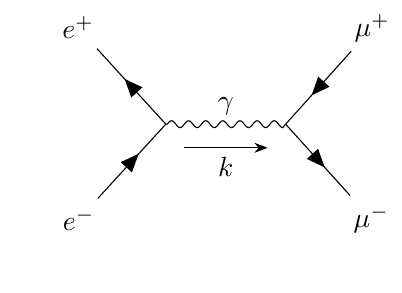
\begin{tikzpicture}
\feynmandiagram [horizontal=a to b] {
i1 [particle=\(e^{-}\)] -- [fermion] a -- [fermion] i2 [particle=\(e^{+}\)],
a -- [photon, edge label=\(\gamma\), momentum'=\(k\)] b,
f1 [particle=\(\mu^{+}\)] -- [fermion] b -- [fermion] f2 [particle=\(\mu^{-}\)],
};
\end{tikzpicture}
        \end{figure}
        \vspace{1cm}
        \begin{center}
           \Large \texttt{\textbf{{\LARGE  S}agnik {\LARGE S}eth }}
        \end{center}
        \vspace{0.5cm}
      \begin{center}
    \textbf{ Dept of Physical Sciences} \\
    \textbf{IISER Kolkata}
    \vspace{0.5cm}

    % Side-by-side logos
   
\end{center}

\end{titlepage}

  
       
\tableofcontents
\newpage
\include{Two_particle}
\end{document}